\documentclass[a4paper]{article}

\pagenumbering{arabic}

\usepackage{mathrsfs}
\usepackage{amsmath}
\usepackage{graphicx}
\usepackage{epstopdf}

\begin{document}

\begin{titlepage}
  \title{Mathematics behind the scaling:\\ From MOSFET to FinFET and beyond}\\
  \author{Aritra~Bhattacharjee\\Sr. Design Engineer, Cadence Design Systems Pvt. Ltd.\\aritrabhattacharjee12@gmail.com, +91-7338133250}
  \date{\today}

  \maketitle
\end{titlepage}

%% Start of the variable defination for the docuent
\def \GL {\textbf{Gauss's Law }}
\def \PE {\textbf{Poisson's equation }}
\def \divD {\nabla \mathcal{D}}
\def \divE {\nabla E}
\def \peX {\frac {d^2\phi} {dx^2}}
\def \peY {\frac {d^2\phi} {dy^2}}
\def \peZ {\frac {d^2\phi} {dz^2}}
\def \peC {\frac{qN_A} {\epsilon_{Si}}}
\def \pe {\peX + \peY + \peZ = \peC}
\def \GLstate {\textit{``The total flux outgoing from a volume is the sum of the charge density inside the volume''}}
\def \PEstate {\textit{the relation between \textbf{potential} at any point in channel with the \textbf{doping} concentration}}
\def \m {\frac{\epsilon_{ox}}{\epsilon_{Si}t_{Si}t_{ox}}}
\def \m1 {\frac{\epsilon_{Si}t_{Si}t_{ox}}{\epsilon_{ox}}}
\def \l {\sqrt{{\frac{\epsilon_{ox}}{\epsilon_{Si}t_{Si}t_{ox}}}}}
\def \H {H_{fin}}
\def \W {W_{fin}}
%% End of the variable defination

\section*{Preface}

\textit{``Behind every successful man, there is a woman.''}\\

The above phrase extends beyond the realms of social life. Like a woman is behind the success of her man, behind the success of the semiconductor physics, there is mathematics.\\

Hailing from a Layout Engineering background I stumble upon a lot of confusion every day. There is a limited access of the data from the Fabrication Lab. There are restrictions from the customer about the product details. The CAD tools simplifies our lives but using these tools makes us forget about the basic concepts of deriving things.\\

I started writing \textbf{``Mathematics behind the scaling: From MOSFET to FinFET and beyond''} to clear some air about these cosfusion regarding scaling.\\

Scaling is an continuous effort from the VLSI industry to generate faster, better and cheaper ICs. As we move below Gate Length of 32nm the Basic MOS structure needs to be modified. The physical reason is explained in many places. But to understand the phenomenon correctly we need to understand the mathematics too. From the mathematical equation, we would be able to make out the reasons behind the changing of the MOS structure required for scaling.\\

This article focuses on the classical approach to derive the scaling equation. The quantum theories of MOSFET is beyond the scope of this article.\\

In this article, first I focus on the derivation of the \PE. Then I illustrate the \PE in MOS. After that we will see the derivation of \PE in MOSFET followed by FinFET. After this point we will get a clear idea about the scaling strategy of beyond FinFET.\\

I hope my midnight fuel is worth your time.
\pagebreak

\section{\PE}
\label{sec:poisson}
To Explain the mathematics behind the semiconductor scaling, we first need to analyze the \PE.
In this section we try to derive the \PE from \GL.

The \GL states that: \GLstate.\\
The mathematical form of the \GL is:

\begin{equation}
  \label{eq:gl}
  \divD = \rho
\end{equation}

Where $\divD$ is the divergent of the flux line and $\rho$ is the charge density within the volume.

Now for the semiconductor devices, the field is caused by the Eclectic flux lines only. This derives the equation \ref{eq:gl}:

\begin{equation}
  \mathcal{D} = \epsilon E\\
\end{equation}
\begin{equation}
  \label{eq:divE}
  \divE = \frac{\rho}{\epsilon}
\end{equation}

For Semiconductor:

\begin{equation}
  \epsilon = \epsilon_{Si}
\end{equation}

In general the total charge density inside of a semiconductor is:

\begin{equation}
  \label{eq:charge}
  \rho = q(p - n + N_D - N_A)
\end{equation}

For the channel region, at inversion stage, only the acceptor ions will be present. Thus the charge density in equation \ref{eq:charge} becomes:

\begin{equation}
  \label{eq:Si-charge}
  \rho = - qN_A
\end{equation}

We know that,

\begin{equation}
  \label{eq:E-phi}
  E = - \nabla \mathcal{\phi}
\end{equation}

Substituting these values from equation \ref{eq:Si-charge} and \ref{eq:E-phi} to equation \ref{eq:divE} we get:

\begin{equation}
  \nabla^2 \phi = - \rho
\end{equation}

Expanding the divergent we get:

\begin{equation}
  \label{eq:pe}
  \pe
\end{equation}

The equation \ref{eq:pe} is known as the \PE. This equation denotes \PEstate.

\section{Illustration of \PE in MOSFET}
\label{sec:Poisson-in-MOS}
In the Section \ref{sec:poisson} we have derived the \PE. In this section we will try to illustrate the \PE in MOSFET.\\

To understand the mathematical form of \PE, first we take a point inside n-chnnel MOSFET. The Elfield field experienced by the point in $x$, $y$ and $z$ Dimensions are $E_x$, $E_y$ and $E_z$ respectively. Refer to figure \ref{fig:E-Field-in-channel} for better understanding.

\begin{figure}[h!]
  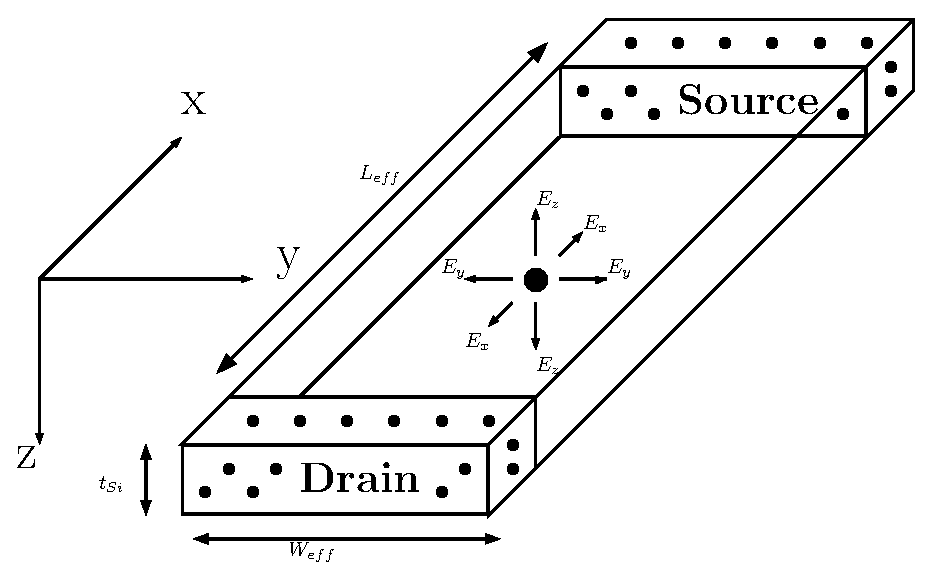
\includegraphics[scale=0.8]{./BulkFinFET-EField-in-Channel.eps}
  \caption{Electric Field in MOSFET Channel}
  \label{fig:E-Field-in-channel}
\end{figure}

From the Figure \ref{fig:E-Field-in-channel} we can observe that, $E_z$ component of the Electric filed is responsible for the Gate Electric Field. The $E_x$ field is Electric field experinced by the point, due to Electric field from Drain to Source. The $E_y$ component will be zero for Single/Double gate MOSFET. This makes the \PE as following:

\begin{align*}
  \pe\\
  Since, \peY = 0\\
  \peX + \peZ = \peC
\end{align*}

Now, we can observe that $\peZ$ is the desired as it occurs due to $E_z$, the Gate Electric Field. The $\peX$ component causes (SCE) Short Channel Effects, such as, DIBL (Drain Induced Barier Lowering). The $\peC$ is a constant. Thus if we can increase the other component $\peZ$, in the \PE, then $\peX$ will come down i.e. will decrease the DIBL effect in the MOSFET. We can achive this by, somehow placeing a gate polysilicon beneath the channel region. This brings the concept of double gate MOSFET. See the figure \ref {fig:MOS-DGMOS} for better visualization\\

\begin{figure}[h!]
  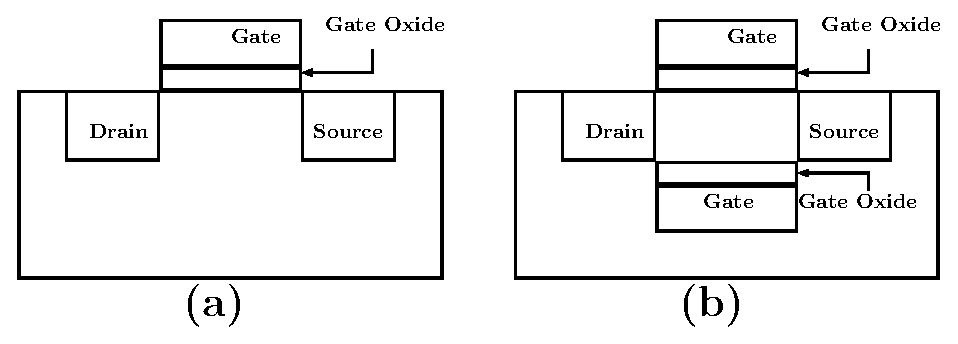
\includegraphics[scale=0.8]{./BulkFinFET-bulk-MOSFET.eps}
  \caption{(a) Bulk MOSFET (b) Double Gate MOSFET}
  \label{fig:MOS-DGMOS}
\end{figure}

\begin{figure}[h!]
  \includegraphics[scale=0.8]{./BulkFinFET-PD-FD-SOI.eps}
  \caption{SOI MOSFET (a) PDSOI Partially Depalted SOI MOSFET (b) FDSOI Fully Depalted SOI MOSFET}
  \label{fig:PDSOI-FDSOI}
\end{figure}

\begin{figure}[h!]
  \includegraphics[scale=0.8]{./BulkFinFET-FinFET.eps}
  \caption{(a) Double Gate Bulk FinFET (b) Tri-Gate Bulk FinFET}
  \label{fig:FinFET}
\end{figure}


From figure \ref {fig:MOS-DGMOS}, we can understand, if we want to decrease the SCE, somehow we need to place a gate at the both sides of the Channel. This brings us some new types of MOS configurations:

\begin{enumerate}
\item \textbf{SOI MOSFET}\\
  SOI stands for Silicon On Insulator. If we look closely in the Double Gate MOS, we will find that beneath the channel, the Gate is responsible for the Electric Field in Channel. Now If we build the MOS Source, Drain and Channel above the $SiO_2$, we can Bias the Bulk Silicon to act like the Second Gate. This way $E_z$ will be increased, thus decreasing the SCE.\\

  There are fair amount of study ongoing with SOI MOSFET. SOI MOSFETs have 2 main varients, depending on the Channel Si height:
  \begin{enumerate}
  \item \textbf{PDSOI}\\
    Partially Deplated SOI MOSFET where the Souce, Drain and Channel width is kept higher. In this configuration, the channel is not fully deplated, and can cause `history error'.
  \item \textbf{FDSOI}\\
    Fully Deplated SOI MOSFET where the Souce, Drain and Channel width is sufficient to make the channel fully depalted. This type of MOSFETs are further optimized by making `Burried Oxide thinner', creating a `ground plane' below the channel. Figure \ref{fig:PDSOI-FDSOI} shows the 2 types of the SOI MOSFETs.
  \end{enumerate}

\item \textbf{FinFET}\\
  Now placing a Gate eletrode beneth the channel is difficult to fabricate. So the Fabrication Porcess was aligned by raising the silicon itself and placing the gate eletrode on both side of the Si. The Si structure looks like a `Fin'. So the device is called the `FinFET'.\\

  Depending on the Structure and the fabrication process, FinFETs can be various type:
  \begin{enumerate}
  \item \textbf{Double gate FinFET}\\
    In this type, both left and right side of the Fins have Gate. Top Side of the Si is unused as it is protected by a hard mask layer.
  \item \textbf{Triple gate FinFET}\\
    In this type, Top side of the Fin is also having the Gate. Thus each of the Fins now have 3 gates, hence the name. Refer to Figure \ref{fig:FinFET} for better visualization.
  \item \textbf{SOI FinFET}\\
    This type os the FinFET is build on the SOI wafer. So this type of FinFET has all the advantages of the SOI as well as FinFET. Unfortunately SOI FinFET process is very expensive as, SOI wafers are expensive than normal bulk Si wafer and for FinFET to fabricate, we need a seperate Mask.
  \end{enumerate}
\end{enumerate}


\section{Solving \PE in MOSFET}

Let us solve the \PE in Single Gate Bulk MOSFET.\\

The controlling Gate Electric filed in MOSFET will only induce $E_z$. The $E_x$ is the unwanted Electric field from Source to Drain. The $E_y$ will not be present as there are not Gate Electrode at the $y$ coordinate. Refer to figure \ref{fig:E-Field-in-channel} in page \pageref{fig:E-Field-in-channel} for better visulization.


\begin{align*}
  The~\PE, \pe\\
  Since, \peY = 0\\
  \peX + \peZ = \peC
\end{align*}

A Solution for the potential $\phi(x,z)$ will be a parabolic form, it can be writen as:

\begin{equation}
  \label{eq:pe-for-MOSFET}
  \phi(x,z) = C_1(x) + C_2(x)z  + C_3(x)z^2
\end{equation}

To solve the equation \ref{eq:pe-for-MOSFET} we need to define some boundary conditions.

\begin{enumerate}
\item At z=0, or $\phi(x,0)$ we define the front surface potential is $\phi_f(x)$. From the equation \ref{eq:pe-for-MOSFET}, this boundary condition translates to:
  \begin{equation}
    \label{eq:MOS-b-cond-1}
    C_1(x)=\phi_f(x)
  \end{equation}
\item The Electric Flux line entering from the Gate Electrode, is passed through the silicon di-oxide Layer to enter the top surface of Silicon bulk. In other words, the Field at the Gate is same as the Field at the Front surface of the Silicon.
  \begin{align*}
    \mathcal{D_{G}} = \mathcal{D_{S}}\\
    \epsilon_{ox} \mathcal{E_{G}} = \epsilon_{Si} \mathcal{E_{S}}\\
    \because \mathcal{E_{S}} = \frac{d\phi}{dz} \bigg\vert_{z=0}\\
    \therefore \frac{d\phi}{dz} \bigg\vert_{z=0} = \frac {\epsilon_{ox}} {\epsilon_{Si}} \mathcal{E_{G}}\\
    Now, \mathcal{E_{G}} = - \frac{\partial V}{\partial x}\\
    \therefor \mathcal{E_{G}} = - \frac{V_{GS}^{'} - \phi_f(x)}{t_{ox}}\\
    So, \frac{d\phi}{dz} \bigg\vert_{z=0} = \frac {\epsilon_{ox}} {\epsilon_{Si}} \frac{\phi_f(x) - V_{GS}^{'}}{t_{ox}}\\
    Where, V_{GS}^{'} = V_{GS} - V_{FBf}
  \end{align*}

In the above expression, the $V_{GS}$ is the voltage difference at the gate oxide, which is applied $V_{GS}$ minus the $V_{FBf}$. $V_{FBf}$ is the Flat Band Voltage at the front surface.\\

The above expression gives us the second variable as:

\begin{equation}
  \label{eq:MOS-b-cond-2}
  \frac{d\phi}{dz} \bigg\vert_{z=0} = C_2(x) = \frac {\epsilon_{ox}} {\epsilon_{Si}} \frac{\phi_f(x) - V_{GS}^{'}}{t_{ox}}
\end{equation}

\item We take the thickness of the Si $t_{Si}$ such that, at $t_{Si}$ depth, there will be no effect of the Electric field.

  \begin{align*}
    \frac{d\phi}{dz} \bigg\vert_{z=t_{Si}} \cong 0\\
    C_2(x) + 2t_{Si}C_3(x) = 0\\
    C_3(x) = - \frac{C_2(x)}{2t_{Si}}
  \end{align*}

  This gives us the third boundary condition:

  \begin{equation}
    \label{eq:MOS-b-cond-3}
    C_3(x) = -\frac{1}{2t_{Si}} \frac {\epsilon_{ox}} {\epsilon_{Si}} \frac{\phi_f(x) - V_{GS}^{'}}{t_{ox}}
  \end{equation}
\end{enumerate}

Now let us put these boundary condition to the equation \ref{eq:pe-for-MOSFET},

\begin{align*}
    \phi(x,z) = C_1(x) + C_2(x)z  + C_3(x)z^2\\
    \phi(x,z) = \phi_f(x) + \frac {\epsilon_{ox}} {\epsilon_{Si}} \frac{\phi_f(x) - V_{GS}^{'}}{t_{ox}}z - \frac{1}{2t_{Si}} \frac {\epsilon_{ox}} {\epsilon_{Si}} \frac{\phi_f(x) - V_{GS}^{'}}{t_{ox}}z^2
\end{align*}

Let us put this value back to the \PE in our single gate MOSFET,

\begin{align*}
  \peX + \peZ =\peC\\
  \frac{d^2\phi_f(x)}{dx^2} \left(1 + \frac{\epsilon_{ox}}{\epsilon_{Si}t_{ox}}z - \frac{\epsilon_{ox}}{2t_{Si}\epsilon_{Si}t_{ox}}z^2\right) - \frac{\epsilon_{ox}}{\epsilon_{Si}t_{Si}t_{ox}}\left( \phi_f(x) - V_{GS}^{'}\right) = \peC
\end{align*}

This solution is valid for all valus of the $z$. Putting $z=0$ in the above equation, we get:

\begin{equation}
  \label{eq:pe-phi-x-in-MOS}
  \frac{d^2\phi_f(x)}{dx^2} - \frac{\epsilon_{ox}}{\epsilon_{Si}t_{Si}t_{ox}}\left( \phi_f(x) - V_{GS}^{'}\right) = \peC
\end{equation}

Let us define a term:

\begin{equation}
  \label{eq:varphi-x}
  \varphi(x) = \phi_f(x) - V_{GS}^{'} +\peC \m1
\end{equation}

Putting the values of equation \ref{eq:varphi-x} into equation \ref{eq:pe-phi-x-in-MOS} we get:

\begin{equation}
  \label{eq:pe-varphi-x-in-MOS}
  \frac{d^2\varphi(x)}{dx^2} - \frac{\epsilon_{ox}}{\epsilon_{Si}t_{Si}t_{ox}} \varphi(x) = 0
\end{equation}

To solve the equation \ref{eq:pe-varphi-x-in-MOS} we need to solve its characteristics equation first. This differential equation is a \textbf{second order} differential equation with \textbf{power 1}. The characteristics equation of this differential equation is as:


\begin{align*}
  m^2 - \frac{\epsilon_{ox}}{\epsilon_{Si}t_{Si}t_{ox}} = 0\\
  \therefore m = \pm \l
\end{align*}
Let us define a term $\lambda_{MOS} = \l$. So the solution to the equation \ref{eq:pe-varphi-x-in-MOS} becomes as:

\begin{equation}
  \label{eq:pe-varphi-solved-MOS}
  \varphi(x) = \varphi_0 \exp\left({\pm x \lambda_{MOS}}\right)
\end{equation}

In the equation \ref {eq:pe-varphi-solved-MOS} the term $\varphi_0$ is a constant. Let us find out the value of the $\varphi_0$.

\begin{equation}
  \label{eq:varphi-0-vbi}
  We~know,~at~x=0, \phi_f(x)=\phi_f(0)=V_{bi}=\varphi_0
\end{equation}

Where $V_{bi}$ is the built in potential of the MOS. This makes the final expression of the front surface potential as:

\begin{equation}
  \label{eq:f-potnetial-of-MOS}
  \phi_f(x) = V_{bi} \exp \left({\pm x \lambda_{MOS}}\right) + V_{GS}^{'} - \peC \frac{1}{\lambda_{MOS}^2}
\end{equation}

This front surface potential will play a pivotal role in determining the short channel effects. As the front surfae potential comprises of the $x$ dependent term, it will depict the variation of the electric field along the channel at the surface of the MOSFET. From this analogy, we will have an understanding of how we should scale in order to elliminate the short channel effects.

\section{Surface Potential of MOSFET}

The surface potential of the MOS is important for discussing the scaling. As the surface potential is a function of $x$, along the channel it will depict the impact of the source and drain. The impact of the drain and or source should be minimal for MOS to operate. In this section we will plot the surface potential of MOS and try to explain in physical term.

Lets start with the equation \ref{eq:f-potnetial-of-MOS}:

\begin{align*}
  \phi_f(x) = V_{bi} \exp \left({\pm x \lambda_{MOS}}\right) + V_{GS}^{'} - \peC \frac{1}{\lambda_{MOS}^2}\\
  At~x=0,~\phi_f(0) = V_{bi} + V_{GS}^{'} -\peC \frac{1}{\lambda_{MOS}^2}\\
  At~x=L_{eq},~\phi_f(L_{eq})  = V_{bi} + V_{DS} + V_{GS}^{'} -\peC \frac{1}{\lambda_{MOS}^2}
\end{align*}

At Drain end, the potential will be $V_{DS} + V_{bi}$. This defines the initail and final valuess of the surface potential. At the channel, as the surface potential is an $x$ dependant term, it will die out. This is true, as the point in channel, will have minimal influence from source or drain.

Since we considered the starting point of the $x$ axis is the source, we reached a surface potential solution as:

\begin{equation}
  \phi_f(x) = V_{bi} \exp \left({\pm x \lambda_{MOS}}\right) + V_{GS}^{'} - \peC \frac{1}{\lambda_{MOS}^2}
\end{equation}

If we star the solution from the source end, we will reach the solution as :

\begin{equation}
  \phi_f(x) = (V_{bi} + V_{DS}) \exp \left({\pm x \lambda_{MOS}}\right) + V_{GS}^{'} - \peC \frac{1}{\lambda_{MOS}^2}
\end{equation}


\section{Solving \PE in FinFET}

To solve the \PE in FinFET, we need to take a closer look into the FinFET structure. From the Figure \ref{fig:FinFET-E-Field} the Gausian Surface is imagine at the FinFET channel region. Inside this Region, a point Experiences the electric Field $E_x$, $E_y$ and $E_z$. $E_x$ is caused by the SCE. $E_z$ is caused by the top Gate. $E_y$ is due to both side of the Gates.

\begin{figure}[h!]
  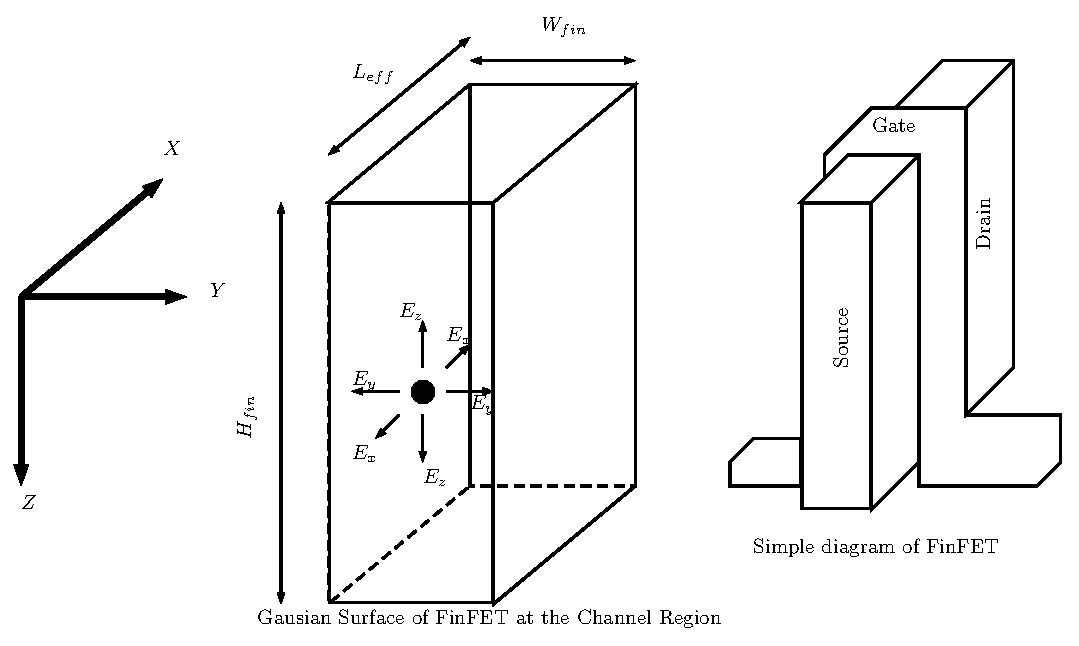
\includegraphics[scale=0.8]{./FinFET-E-Field.eps}
  \caption{Tri-Gate Bulk FinFET with Gausian surface at the Channel region}
  \label{fig:FinFET-E-Field}
\end{figure}

We know, that \PE is:

\begin{equation}
  \pe
\end{equation}

Now the Gate is causing the $E_z$ and $E_y$ electric Fields. If the FinFET structure are a perfect cube, then the $E_y$ would be 2 times of $E_z$. Since the width and the height are \W and \H respectively, the electric field will be:

\begin{align*}
  E_y = \frac{2\H}{\W} E_z
\end{align*}

This makes the \PE to become:

\begin{equation}
  \label{eq:pe-finFET}
  \peX + \left( 1 + \frac{\W}{2 \H} \right) \peY = \peC
\end{equation}

Now, like MOSFET equation \ref{eq:pe-for-MOSFET}, the FinFET surface potential solution can be approzimated as:

\begin{equation}
  \label{eq:fin-pe-cond}
  \phi(x,y) = C_1(x) + C_2(x)y  + C_3(x)y^2
\end{equation}

Let us consider the boundary conditions for solving the equation \ref{eq:fin-pe-cond}.

\begin{enumerate}
\item At $y=0$ and at $y=t_{Si}$, let, the surface potential be, $\phi_f(x)$. This makes the first Boundary condition:
  \begin{equation}
    \label{eq:fin-cond-1}
    C_1(x)=\phi_f(x)
  \end{equation}
\item At $y=0$, the Electric flux lines from the Gate Oxide will enter the Silicon Surface at the channel region. Like the MOSFET, this will make the Electric Field as:
  \begin{align*}
    So, \frac{d\phi}{dy} \bigg\vert_{y=0} = \frac {\epsilon_{ox}} {\epsilon_{Si}} \frac{\phi_f(x) - V_{GS}^{'}}{t_{ox}}\\
    Where, V_{GS}^{'} = V_{GS} - V_{FBf}
  \end{align*}
  The second Boundary Condition becomes as:
  \begin{equation}
    \label{eq:fin-cond-2}
    C_2(x)=\frac {\epsilon_{ox}} {\epsilon_{Si}} \frac{\phi_f(x) - V_{GS}^{'}}{t_{ox}}
  \end{equation}
\item At $y=\W$, same gate electric field will be applied as at $y=0$. This will make:
  \begin{align*}
    \mathcal{D_{G}} = - \mathcal{D_{S}}\\
  \end{align*}
  The - sign comes as this electric field is opposite to the direction of the axis consideration.
  \begin{align*}
    \epsilon_{ox} \mathcal{E_{G}} = - \epsilon_{Si} \mathcal{E_{S}}\\
    \because \mathcal{E_{S}} = \frac{d\phi}{dy} \bigg\vert_{y=\W}\\
    \therefore \frac{d\phi}{dy} \bigg\vert_{y=\W} = - \frac {\epsilon_{ox}} {\epsilon_{Si}} \mathcal{E_{G}}\\
    Now, \mathcal{E_{G}} = - \frac{\partial V}{\partial x}\\
    \therefor \mathcal{E_{G}} = \frac{V_{GS}^{'} - \phi_f(x)}{t_{ox}}\\
    \frac{d\phi}{dy} \bigg\vert_{y=\W} = - \frac {\epsilon_{ox}} {\epsilon_{Si}} \frac{\phi_f(x) - V_{GS}^{'}}{t_{ox}}
  \end{align*}
  Putting this value to the equation \ref{eq:fin-pe-cond}, we get:
  \begin{align*}
    C_2(x) + 2\WC_3(x)= - C_2(x)\\
    C_3(x) = - \frac{1}{\W} C_2(x)
  \end{align*}
  \begin{equation}
    \label{eq:fin-cond-3}
    C_3(x) = - \frac{1}{\W} \frac {\epsilon_{ox}} {\epsilon_{Si}} \frac{\phi_f(x) - V_{GS}^{'}}{t_{ox}}
  \end{equation}
\end{enumerate}

Putting the Boundary conditions from equation \ref{eq:fin-cond-1}, \ref{eq:fin-cond-2} and \ref{eq:fin-cond-3} in equation \ref{eq:fin-pe-cond}, we get:

\begin{align*}
  \phi(x,y) = C_1(x) + C_2(x)y  + C_3(x)y^2\\
  \phi(x,y) = \phi_f(x) + \frac {\epsilon_{ox}} {\epsilon_{Si}} \frac{\phi_f(x) - V_{GS}^{'}}{t_{ox}} y -  \frac{1}{\W} \frac {\epsilon_{ox}} {\epsilon_{Si}} \frac{\phi_f(x) - V_{GS}^{'}}{t_{ox}} y^2
\end{align*}

Let's substitute this value of $\phi(x,y)$ in equation \ref{eq:pe-finFET}:
\begin{align*}
    \peX + \left( 1 + \frac{\W} {2 \H} \right) \peY = \peC\\
    \frac{d^2\phi_f(x)}{dx^2} \left(1 + \frac{\epsilon_{ox}}{\epsilon_{Si}t_{ox}}y - \frac{\epsilon_{ox}}{\W \epsilon_{Si}t_{ox}}y^2\right) - \left( 1 + \frac{\W}{2 \H} \right) \frac{2 \epsilon_{ox}}{\epsilon_{Si}\W t_{ox}}\left( \phi_f(x) - V_{GS}^{'}\right) = \peC
\end{align*}
This equation is vaid for all values of $y$. At $y=0$, $\phi(x,y)=\phi_f(x)$, the above equation becomes:
\begin{equation}
  \label{eq:fin-pe-at-y0}
  \frac{d^2\phi_f(x)}{dx^2} - \left( 1 + \frac{\W}{2 \H} \right) \frac{2 \epsilon_{ox}}{\epsilon_{Si}\W t_{ox}}\left( \phi_f(x) - V_{GS}^{'}\right) = \peC
\end{equation}

Like MOSFET solution, let us consider a term, $\lambda_{FIN}$, as:

\begin{equation}
  \lambda_{FIN} = \sqrt {\left( 1 + \frac{\W}{2 \H} \right) \frac{2 \epsilon_{ox}}{\epsilon_{Si}\W t_{ox}}}
\end{equation}

Let us consider a term, $\varphi_f(x)$ as:

\begin{equation}
  \varphi_f(x) = \phi_f(x) - V_{GS}^{'} + \peC \frac{1}{\lambda_{FIN}^2}
\end{equation}

This makes equation \ref{eq:fin-pe-at-y0} as:

\begin{equation}
  \label{eq:varphi-fin}
  \frac{d^2\varphi_f(x)}{dx^2} - \lambda_{FIN}^2\varphi_f(x) = 0
\end{equation}

This is a standard \textbf{second order}, \textbf{first degree} differential equation. The standart solution of the equation \ref{eq:varphi-fin} is :

\begin{equation}
  \varphi_f(x) = \varphi_0 \exp(\pm x \lambda_{FIN})
\end{equation}

Like MOSFET, the constant $\varphi_0$ will be $V_{bi}$. This makes the final expression of the FinFET surface potential as:

\begin{equation}
  \phi_f(x) = V_{bi} \exp(\pm x \lambda_{FIN}) + V_{GS}^{'} - \peC \frac{1}{\lambda_{FIN}^2}
\end{equation}

\section{Surface Potential of FinFET}

\section{Comparision of the Surface Potential of MOSFET and FinFET}



\end{document}

